\documentclass[main.tex]{subfiles}
\section{Component Overview}

\subsection{Project Overview}
TODO: WRITE SUBSECTION ABOUT OVERVIEW OF THE TOTAL PROJECT.

\subsection{Image Manipulation Components}
Here follows an implementation of all the subproblems introduced in the previous section.
Before starting with discussing the different sub problems, the objective of this phase is transforming the image to a new image were the following thing has happend: edgde detection to define possible areas where the license plate can be.
To do this, the subproblems defined in the previous section, subsection image manipulation are implemntated.
This implementation is shown in the current sub section.
\subsubsection{Image Preparation}
First steps are making the image uniform and removing the color without losing elements in the picture.
The color removing is called greyscaling. 
In the project is a seperate script present that reads and greyscales the image.
Therefore can subproblems~\vref{sub:uniform} and~\vref{sub:greyscale} be combined when talking about the implemntation.
The matlab code corresponding to these subproblems can be found in listing~\vref{greyscale}.
These subproblems are solved in the custom made matlab function called \textit{[rgbImage,greyImage] = greyscale(inputFileName)}.
This function has an input argument and produces two output products.
As an input the name of the file to read can be found. 
By making this a variables it is easy to change the change the file name, what is only good for the dynamic carater of the application.
When looking at the output arguments, both an rgb and greyscale image can be found.
This happens to keep the original in the system while executing the program.
When looking at the body of this function, the try catch is present to catch any possible error.
Because the project consists of a lot of components, it is a very handy feature to always have a more detailed explenation when the program crashes for one reason or another.
While the first lines take care of the importing of the picture and ashoring that it is an rgb version.
Line 15 in the code solves subproblem~\vref{sub:uniform}. 
The image is resized using the command \textit{imresize()}, from now on all the images are the same size.
The lines 18 to 25 take care of the greyscaling. 
Greyscaling an image is done by seperating the r, g and b channels, multipling each channel by a certain factor and recombining the new value.
New value, as in singluar value, because in a greyscale image are the r,g and b values equal for each pixel.
The factors used can be found in equation~\vref{eq:greyscale}.
\begin{equation}
    Y_{linear} = 0.2126R_{linear} + 0.7152G_{linear} + 0.0722B_{linear}
    \label{eq:greyscale}
\end{equation}
The value of these factors are defined in the \textit{CIE 1931}.
When everything is executed as supposed to, the function now returns both the greyscale and rgb image, otherwise the inputimage is returned twice.
\par
From this point on, a greyscaled image is used in the script.
Before starting with edge detection it is usefull to remove the noise from a picture.
The noise removal is done with the command \textit{medfilt2()}. 
This function also accepts an gpuarray input, this is a better and faster way because the matrix manipulations will be done by the GPU.
The gpu has a significant more cores to calculate results.
The gpu functionality does relie on the CUDA compatability of the gpu in the computer it is running on.
Because this is not generally supported, I made the decision to not go forward with gpu implementation in the standerd version of my project.
With removing the noise, subproblem~\vref{sub:noise} is solved.

\subsubsection{Edge Detection}
After preparing the image, it is now ready to start the edge detection.
Before discussion the implementation, a short explenation what edge detection is and how it can be achieved.
An edge in an image is an area where the rgb pixel values drasticly change. 
For this reason it was important to remove the color without losing any value of the image.
\par
Imagin not using a greyscaled image but a full colored rgb image.
Looking for edges is far more complicated because we have three different channels to take into account.
When using a greyscaled image, the r g and b channels have the same value what makes the detection a lot easier.
One of the most used detection technics is both dilating and erroding the image.
The difference between the two resulting images will result in a very good edge detection.
\par
To succesfull dilate an image, it is necesairy to have a neighborhoud search area, this can be created using a \textit{strel} function.
Imagine to have a neighborhoud that looks like a cicrle with radius of a few pixels. This is shown in figure~\vref{fig:strel}.
\begin{figure}
    \centering
    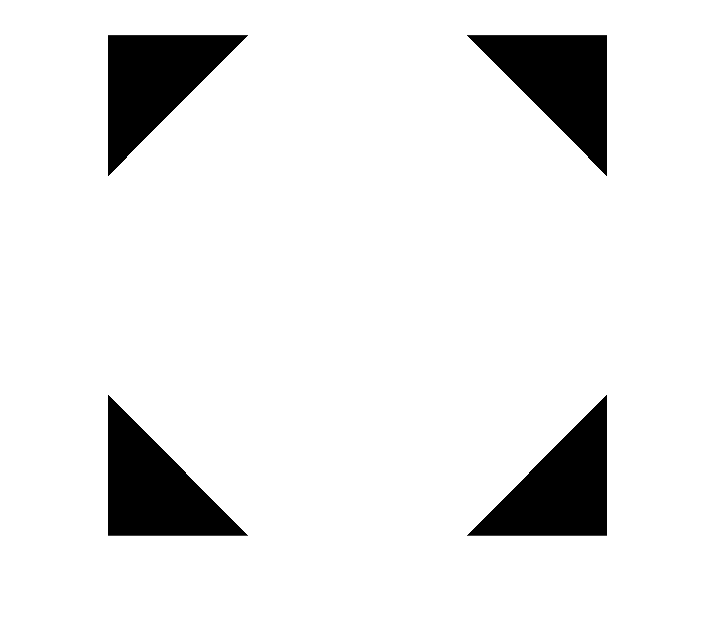
\includegraphics[width=0.7\linewidth]{strel.png}
    \caption{Example of a strel neighborhoud.}
    \label{fig:strel}
\end{figure}
This \textit{strel} is moving over an image, when it covers an aerea with the same rgb value, the system nows it is in an area without a border.
But when the \textit{strel} is in an area that is covered with more than one different value, it is clear that their is a border present.
When there is a pixel of the \textit{strel} that has a lighter value \footnote{Lighter in greyscale value means a higher value} than the center pixel, the value of this center pixel becomes this lighter value.
When this is done on an image, the lighter areas on the image will become bigger.
This is shown in figure~\vref{fig:dilate}.
\begin{figure}
    \centering
    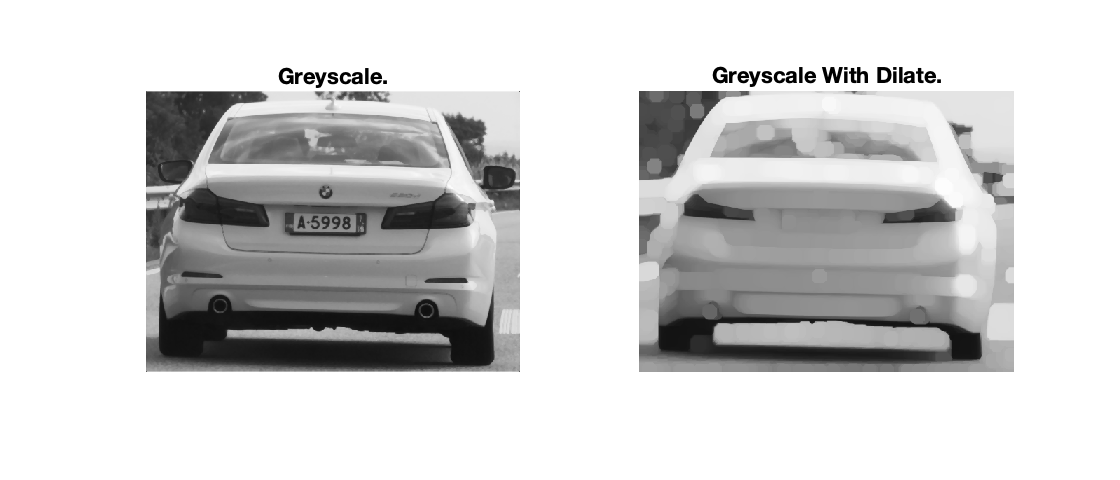
\includegraphics[width=0.9\linewidth]{dilate.png}
    \caption{Example of a dilated image.}
    \label{fig:dilate}
\end{figure}
\par
To succesfull erode an image, it is necesairy to have a neighborhoud search area, this can be created using a \textit{strel} function.
Imagine to have a neighborhoud that looks like a cicrle with radius of a few pixels. This is shown in figure~\vref{fig:strel}.
This \textit{strel} is moving over an image, when it covers an aerea with the same rgb value, the system nows it is in an area without a border.
But when the \textit{strel} is in an area that is covered with more than one different value, it is clear that their is a border present.
When there is a pixel of the \textit{strel} that has a darker value \footnote{Darker in greyscale value means a lower value} than the center pixel, the value of this center pixel becomes this darker value.
When this is done on an image, the lighter areas on the image will become smaller.
This is shown in figure~\vref{fig:erode}.
\begin{figure}
    \centering
    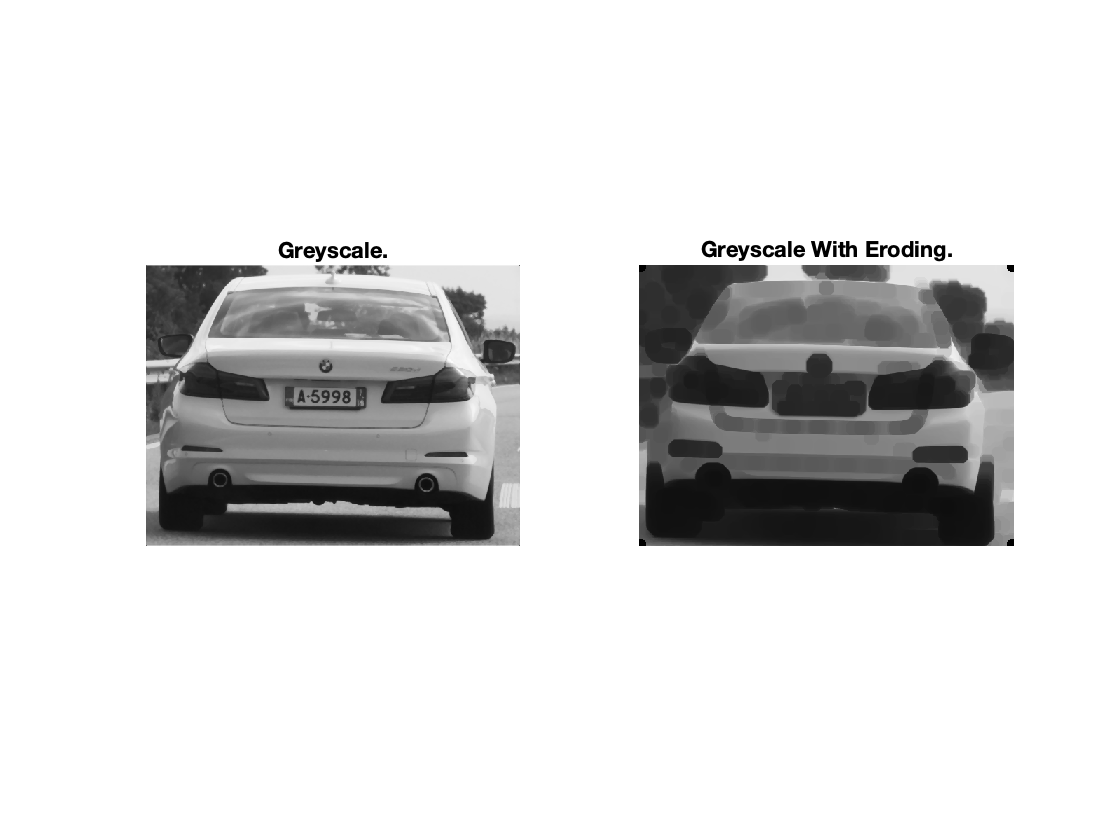
\includegraphics[width=0.9\linewidth]{erode.png}
    \caption{Example of a eroded image.}
    \label{fig:erode}
\end{figure}
\par
In the previous paragraphs, dilating and eroding is exagerated.
When the radius of the \textit{strel} is reduced to 1, the edges can be exact deteremt when the the results are subtracted.
The result of this is shown in figure~\vref{fig:de}.
\begin{figure}
    \centering
    \includegraphics[width=0.9\linewidth]{DE.png}
    \caption{Example of an all edge detection}
    \label{fig:de}
\end{figure}
With this result we can conclude that subproblem~\vref{sub:detectAllEdges} is solved.
\subsubsection{Filling}
